\section{Leistungshalbleiter in der Leistungselektronik}

\subsection{Rolle der Leistungshalbleiter im Energiesystem}

Leistungshalbleiter dienen der verlustarmen, schnellen und steuerbaren Umsetzung elektrischer Energie.
Im Gegensatz zu linearen Bauelementen arbeiten sie nicht im kontinuierlichen Arbeitsbereich,
sondern ausschliesslich als Schalter mit diskreten Zuständen.

Sie besitzen drei Betriebszustände:
\begin{itemize}
\item \textbf{leitend}: Stromfluss mit niedrigem Spannungsabfall,
\item \textbf{sperrend}: Blockieren der angelegten Spannung bis zur maximalen Sperrspannung,
\item \textbf{umschaltend}: Übergangsphase zwischen leitend und sperrend.
\end{itemize}

Damit realisieren sie:
\begin{itemize}
\item Gleichrichtung von Wechsel- zu Gleichspannung,
\item Phasenanschnitt zur Leistungssteuerung,
\item Taktbetrieb bei Gleichstromstellern (PWM),
\item Umrichtung von Spannung, Strom und Frequenz in Umrichtern.
\end{itemize}

Grundlegende Kenngrössen:
\[
U_{RRM},\quad I_{F},\quad U_F,\quad t_{on},\ t_{off},\quad P_{cond},\ P_{sw}.
\]

Dabei bezeichnet $U_{RRM}$ die maximal zulässige Sperrspannung, $I_F$ den maximalen Durchlassstrom
und $U_F$ den Spannungsabfall im leitenden Zustand.
Die Zeiten $t_{on}$ und $t_{off}$ bestimmen die Dauer der Schaltvorgänge.
$P_{cond}$ beschreibt die Leitverluste, $P_{sw}$ die Schaltverluste.

\subsection{Physikalische Grundlagen der Halbleiterbauelemente}

Alle Leistungshalbleiter beruhen auf pn-Übergängen, deren elektrisches Verhalten
durch Dotierung und Feldverteilung bestimmt wird.

Im Sperrbetrieb blockiert der pn-Übergang den Stromfluss:
\[
i \approx 0,\qquad u \le U_{RRM}
\]

Im Durchlassbetrieb ist der pn-Übergang leitend:
\[
i \gg 0,\qquad u \approx U_{on}
\]

Die maximale Sperrspannung wird bestimmt durch:
\begin{itemize}
\item die Dicke der Sperrschicht,
\item die Dotierung der Halbleiterzonen,
\item die elektrische Feldverteilung im pn-Übergang.
\end{itemize}

Thermische Belastung:
\[
\boxed{T_j = T_{amb} + R_{th} \cdot P_V}
\]

Dabei ist $T_j$ die Sperrschichttemperatur, $T_{amb}$ die Umgebungstemperatur,
$R_{th}$ der thermische Widerstand zwischen Sperrschicht und Umgebung
und $P_V$ die im Bauelement entstehende Verlustleistung.
Die Einhaltung von $T_j < T_{j,\max}$ ist zwingend für einen sicheren Betrieb.

\subsection{Diode als Leistungsschalter}

Die Leistungsdiode ist ein ungesteuertes Halbleiterbauelement mit zwei stabilen Zuständen.
Sie leitet Strom in Durchlassrichtung und blockiert in Sperrrichtung.
Sie wird vor allem in Gleichrichtern, Freilaufpfaden und als Schutzbauelement eingesetzt.

\subsubsection{Betriebszustände}

Die Leistungsdiode besitzt zwei stabile Zustände:

\textbf{Durchlass:}
\[
u_D > 0,\qquad i_D > 0
\]

\textbf{Sperre:}
\[
u_D < 0,\qquad i_D \approx 0
\]

Ideales Modell:
\[
u_D =
\begin{cases}
0, & i_D > 0 \\
\infty, & i_D = 0
\end{cases}
\]

\subsubsection{Statisches Durchlassmodell}

Reales Modell:
\[
\boxed{u_D = U_{D0} + r_D \, i_D}
\]

Hier ist $U_{D0}$ der konstante Durchlassspannungsabfall und $r_D$ der differentielle Widerstand
im leitenden Zustand.

Verlustleistung:
\[
\boxed{P_D = U_{D0} \, I_{D,\mathrm{avg}} + r_D \, I_{D,\mathrm{RMS}}^2}
\]

Dabei ist $I_{D,\mathrm{avg}}$ der Mittelwert des Diodenstroms
und $I_{D,\mathrm{RMS}}$ der Effektivwert.

Interpretation:
\begin{itemize}
\item $U_{D0}$ dominiert bei kleinen Strömen,
\item $r_D$ dominiert bei grossen Strömen.
\end{itemize}

\begin{center}
    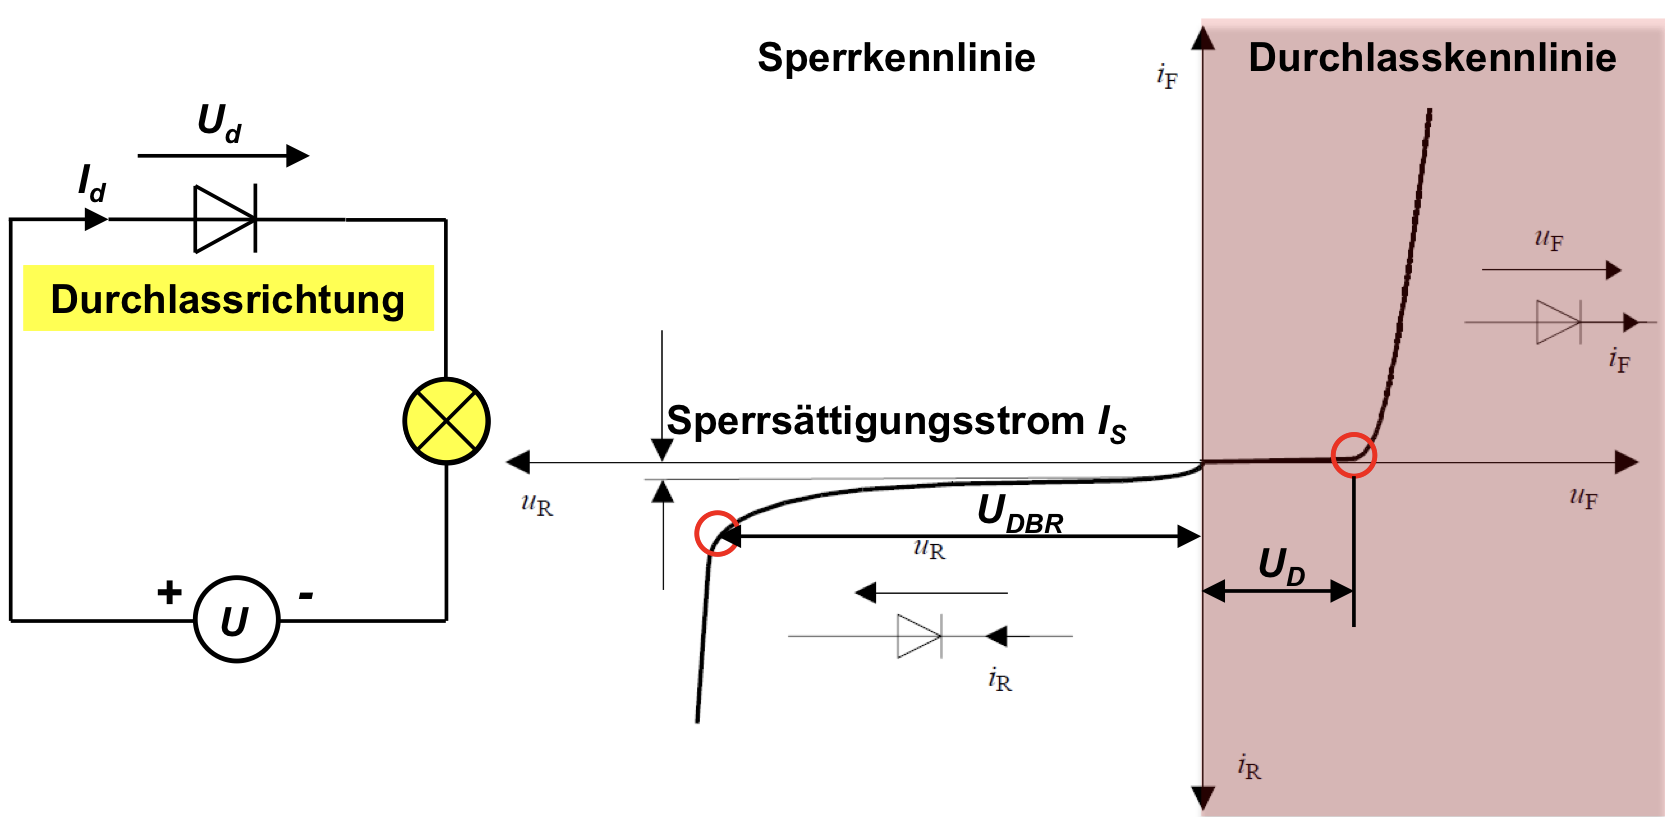
\includegraphics[width=0.85\linewidth]{images/Didodekennlinie.png}
\end{center}
\begin{center}
    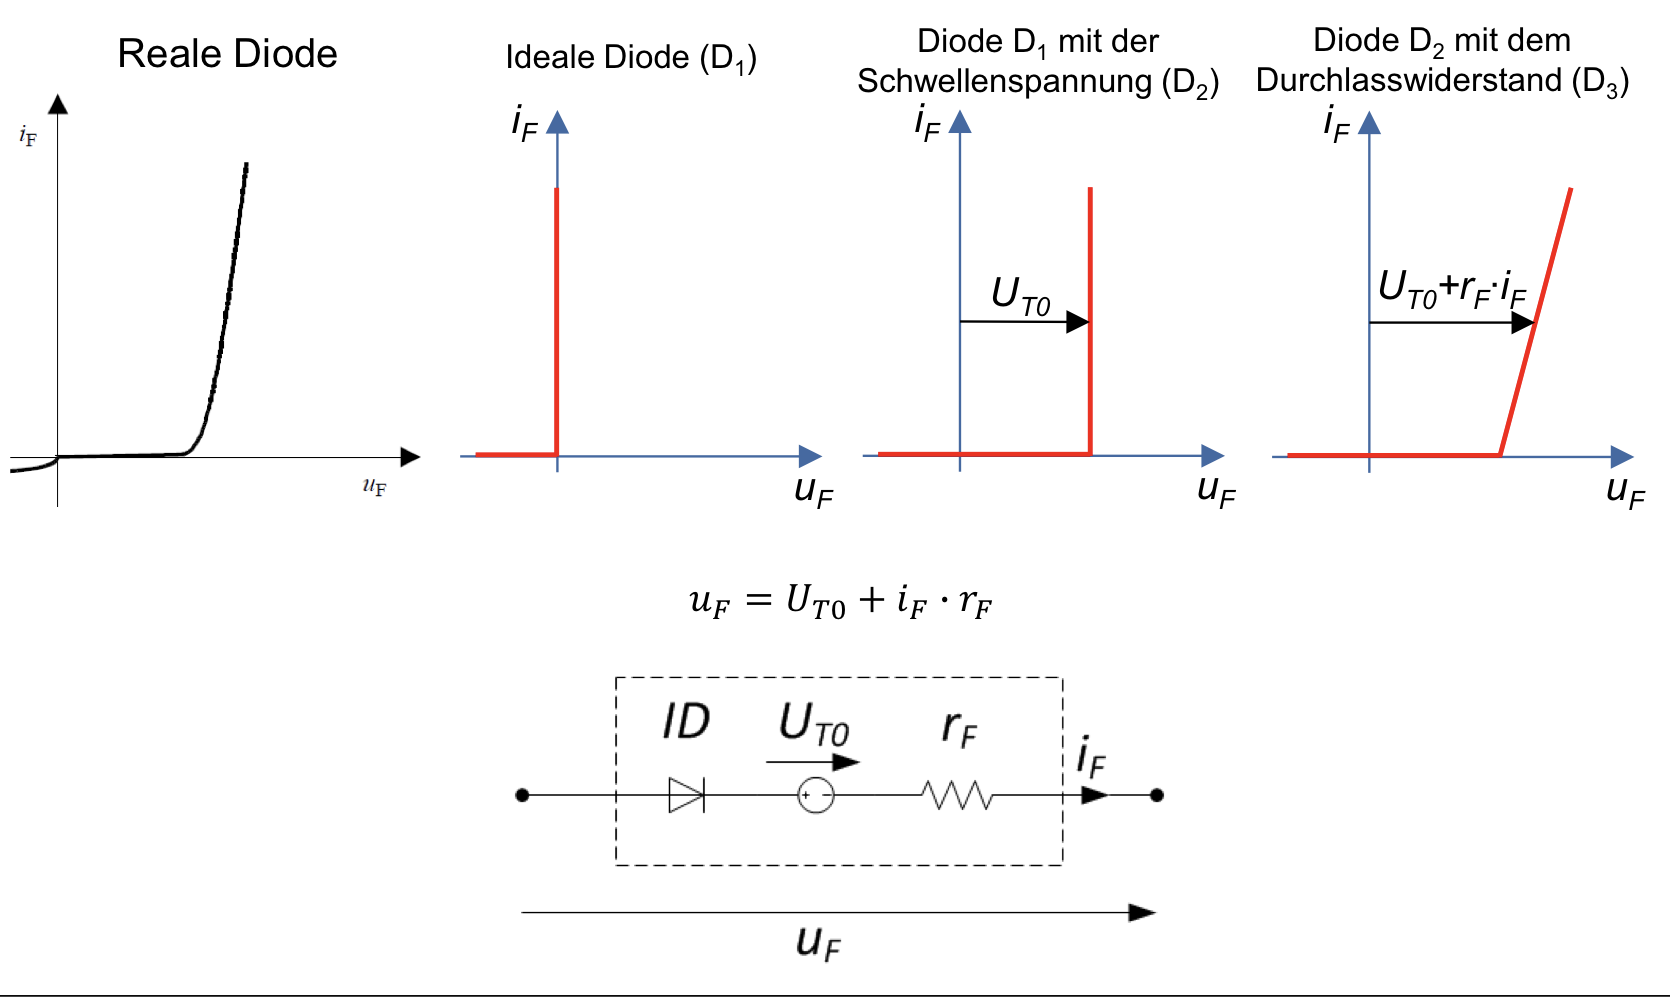
\includegraphics[width=0.85\linewidth]{images/didodeunterschied.png}
\end{center}

\subsubsection{Dynamisches Schaltverhalten}

Beim Übergang von Durchlass nach Sperre muss gespeicherte Ladung aus der Sperrschicht entfernt werden.

Rückerholstrom:
\[
i_{rr}(t)
\]

Rückerholladung:
\[
\boxed{Q_{rr} = \int_0^{t_{rr}} i_{rr}(t)\,dt}
\]

Zusätzliche Schaltverluste:
\[
\boxed{P_{sw,D} \approx f_s \, U_R \, Q_{rr}}
\]

Dabei ist $Q_{rr}$ die gespeicherte Ladung, $f_s$ die Schaltfrequenz
und $U_R$ die anliegende Sperrspannung.

Physikalische Bedeutung:
\begin{itemize}
\item grosse $Q_{rr}$ $\Rightarrow$ hohe Schaltverluste,
\item schnelle Dioden notwendig bei hohen $f_s$.
\end{itemize}

\begin{center}
    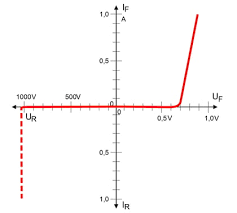
\includegraphics[width=0.85\linewidth]{images/rueckerhol.png}
\end{center}

\subsection{Thyristor (SCR)}

Der Thyristor ist ein gesteuerter, selbsthaltender Leistungsschalter mit PNPN-Struktur.
Er wird durch einen kurzen Gate-Strom gezündet und bleibt leitend,
solange der Anodenstrom oberhalb des Haltestroms liegt.
Ein aktives Abschalten ist nicht möglich.

\subsubsection{Vier-Schichten-Struktur und Zündprinzip}

Der Thyristor besitzt eine PNPN-Struktur.

Zündbedingung:
\[
u_{AK} > 0 \quad \text{und} \quad i_G > 0
\]

Nach dem Zünden:
\[
\boxed{\text{Selbsthaltung durch innere Rückkopplung}}
\]

Haltestrom:
\[
\boxed{i_A > I_H}
\]

Abschalten nur durch:
\begin{itemize}
\item Stromnulldurchgang,
\item externe Kommutierung.
\end{itemize}

\begin{center}
    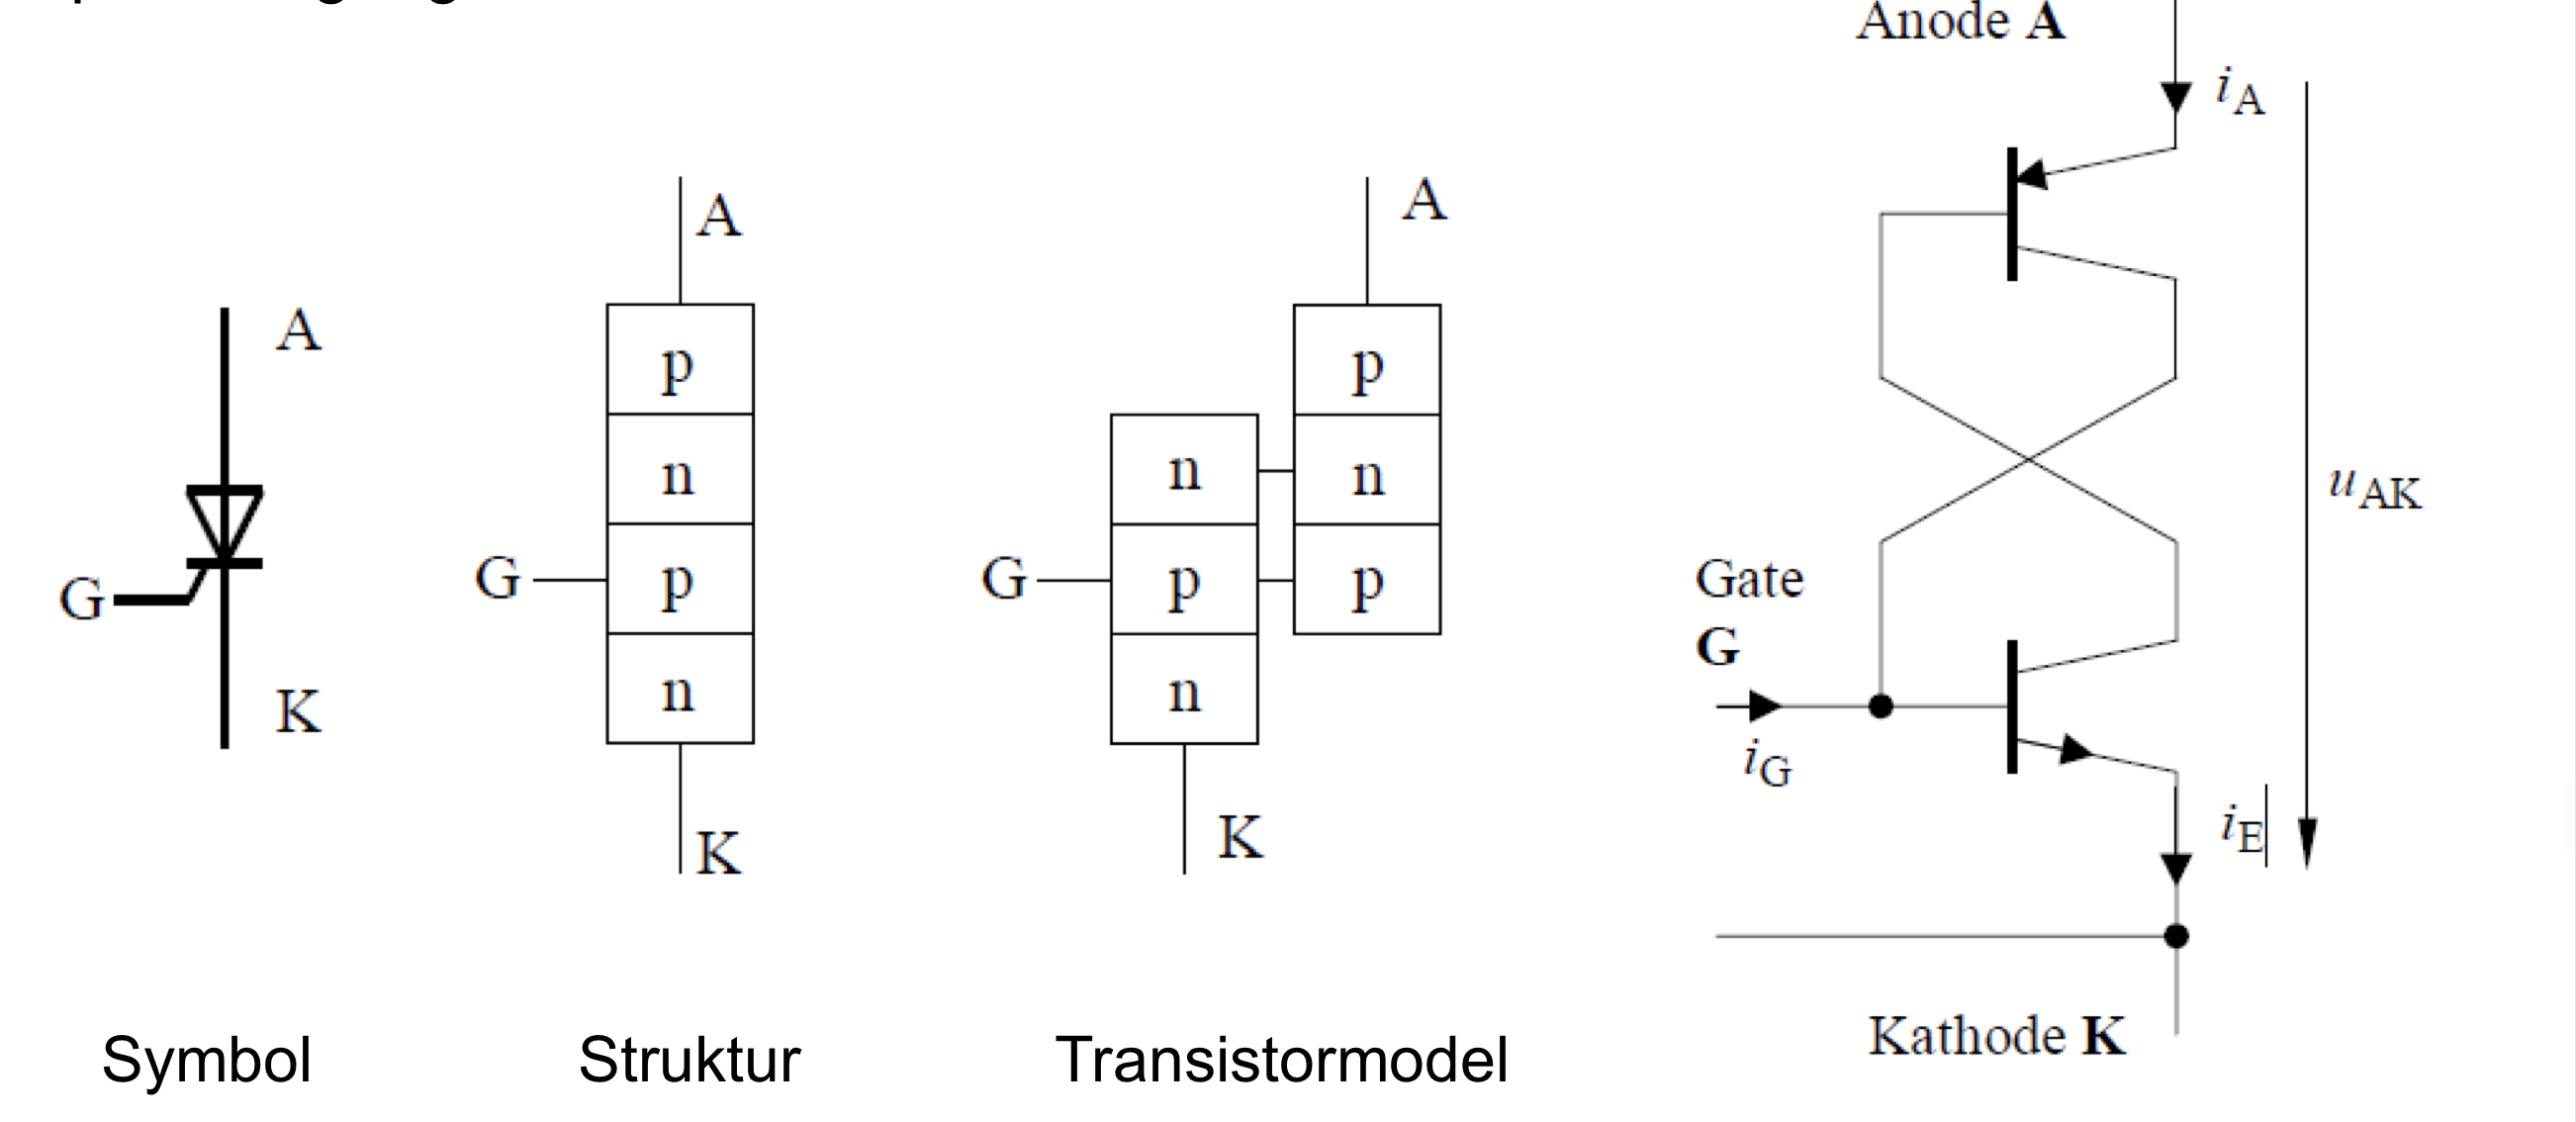
\includegraphics[width=0.85\linewidth]{images/thyristor.png}
\end{center}

\subsubsection{Statisches Modell und Verluste}

\[
\boxed{u_T = U_{T0} + r_T \, i_T}
\]

Hier ist $U_{T0}$ der konstante Durchlassabfall und $r_T$ der differentielle Widerstand.

\[
\boxed{P_T = U_{T0} \, I_{T,\mathrm{avg}} + r_T \, I_{T,\mathrm{RMS}}^2}
\]

Zusätzliche Kenngrössen:
\[
\frac{di}{dt}_{\max},\qquad \frac{du}{dt}_{\max}
\]

Diese Grenzwerte begrenzen die zulässige Strom- und Spannungssteilheit beim Zünden.

Bedeutung:
\begin{itemize}
\item Begrenzen den Zündstromanstieg,
\item Schutz durch Snubber notwendig.
\end{itemize}

\subsection{Leistungs-MOSFET}

Der Leistungs-MOSFET ist ein spannungsgesteuerter Halbleiterschalter.
Er wird über das Gate eingeschaltet und benötigt keinen Gate-Strom im stationären Zustand.
Er eignet sich besonders für hohe Schaltfrequenzen.

\subsubsection{Gate-gesteuerter Feldeffekttransistor}

Leitbedingung:
\[
\boxed{u_{GS} > U_{th}}
\]

Dabei ist $U_{th}$ die Gate-Schwellspannung.

Im leitenden Zustand:
\[
\boxed{u_{DS} = r_{DS,on} \, i_D}
\]

Charakteristisch:
\begin{itemize}
\item Mehrheitsladungsträger,
\item kein Speicherladungseffekt,
\item sehr schnelles Schalten.
\end{itemize}

\begin{center}
    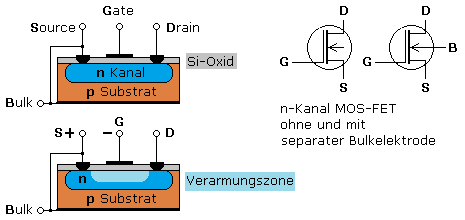
\includegraphics[width=0.85\linewidth]{images/MOSFET.png}
\end{center}

\subsubsection{Dynamisches Modell und Gate-Ladung}

Gate-Ladung:
\[
Q_G = Q_{GS} + Q_{GD}
\]

Dabei ist $Q_G$ die gesamte zum Schalten notwendige Gate-Ladung.

Schaltzeit:
\[
t_{on} \approx \frac{Q_G}{I_G}
\]

Hier bestimmt der verfügbare Gate-Strom $I_G$ die erreichbare Schaltgeschwindigkeit.

Schaltverluste:
\[
\boxed{P_{sw,M} \approx f_s \int u_{DS}(t)i_D(t)\,dt}
\]

\subsection{IGBT}

Der IGBT ist ein hybrides Bauelement aus MOS-Gate und bipolarer Stromleitung.
Er verbindet die einfache Ansteuerung des MOSFET mit den geringen Leitverlusten bipolarer Bauelemente.
Er wird vor allem bei mittleren Schaltfrequenzen und hohen Strömen eingesetzt.

\subsubsection{Hybridstruktur MOS–Bipolar}

Der IGBT kombiniert:
\begin{itemize}
\item spannungsgesteuertes MOS-Gate,
\item stromtragende bipolare Struktur.
\end{itemize}

Leitbedingung:
\[
\boxed{u_{GE} > U_{th}}
\]

Durchlassmodell:
\[
\boxed{u_{CE} = U_{CE0} + r_{CE} \, i_C}
\]

\begin{center}
    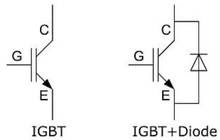
\includegraphics[width=0.85\linewidth]{images/IGBT.png}
\end{center}

\subsubsection{Tail-Strom und Abschaltverluste}

Beim Abschalten verbleibt gespeicherte Ladung im Driftgebiet.

Tail-Strom:
\[
i_{tail}(t)
\]

Zusätzliche Verluste:
\[
\boxed{P_{off} \gg P_{on}}
\]

Konsequenz:
\begin{itemize}
\item langsamer als MOSFET,
\item dafür geringere Leitverluste bei grossen Strömen.
\end{itemize}

\subsection{Vergleich der Bauelemente}

\begin{center}
\begin{tabular}{l|c|c|c|c}
 & Diode & Thyristor & MOSFET & IGBT \\
\hline
Steuerbar & nein & Zünden & ja & ja \\
Abschaltbar & ja & nein & ja & ja \\
Schaltfreq. & mittel & tief & sehr hoch & mittel \\
Leitverluste & klein & klein & klein bei klein $I$ & klein bei gross $I$ \\
Speicherladung & ja & ja & nein & ja \\
\end{tabular}
\end{center}

\subsection{Safe Operating Area (SOA)}

Die Safe Operating Area beschreibt den zulässigen Arbeitsbereich eines Leistungshalbleiters
im Strom--Spannungs--Diagramm.

Zulässige Grenzbedingungen:
\[
\boxed{
\begin{aligned}
u &< U_{RRM} \\
i &< I_{\max} \\
P &= u \cdot i < P_{\max} \\
\frac{di}{dt} &< \left(\frac{di}{dt}\right)_{\max} \\
\frac{du}{dt} &< \left(\frac{du}{dt}\right)_{\max}
\end{aligned}
}
\]

Physikalische Bedeutung:
\begin{itemize}
\item Begrenzung durch Durchbruchspannung,
\item Begrenzung durch thermische Überlast,
\item Begrenzung durch sekundären Durchbruch.
\end{itemize}

Die Einhaltung der SOA ist zwingend für den sicheren Betrieb.

\subsection{Zusammenfassung der Verlustmechanismen}

Gesamtverluste:
\[
\boxed{P_V = P_{cond} + P_{sw}}
\]

Dabei beschreibt $P_{cond}$ die Verluste im leitenden Zustand
und $P_{sw}$ die Verluste während der Schaltvorgänge.

\[
P_{cond} = U_0 I_{\mathrm{avg}} + r I_{\mathrm{RMS}}^2
\]
\[
P_{sw} = f_s \int u(t)i(t)\,dt
\]

Thermische Auslegung:
\[
T_j = T_{amb} + R_{th} P_V < T_{j,\max}.
\]

\subsection{Vereinfachte Schaltverlustrechnung}

Bei näherungsweise linearem Spannungs- und Stromverlauf während des Schaltens gilt:

\paragraph{Einschaltverlust}

\[
\boxed{E_{on} \approx \frac{1}{2} U \, I \, t_{on}}
\]

\paragraph{Ausschaltverlust}

\[
\boxed{E_{off} \approx \frac{1}{2} U \, I \, t_{off}}
\]

Mittlere Schaltverluste:

\[
\boxed{
P_{sw} = f_s \left(E_{on} + E_{off}\right)
}
\]

Konsequenzen:
\begin{itemize}
\item $f_s \uparrow \Rightarrow P_{sw} \uparrow$
\item $t_{on}, t_{off}$ klein $\Rightarrow$ geringe Verluste.
\end{itemize}

\subsection{Thermische Widerstandskette}

\[
\boxed{R_{th,tot} = R_{th,jc} + R_{th,ck} + R_{th,ka}}
\]

Temperaturen:

\[
T_j = T_{amb} + R_{th,tot} P_V
\]
\[
T_c = T_j - R_{th,jc} P_V,
\qquad
T_k = T_c - R_{th,ck} P_V
\]

Grenzbedingung:
\[
\boxed{T_j < T_{j,\max}}
\]
